\lab{Bifurcations and Hysteresis}{Bifurcations and Hysteresis}
\label{lab:Bifurcations}
\labdependencies{IVPBVPIntro}

Recall that any ordinary differential equation can be written as a first order system of ODEs,
\begin{align}
x' = F(x), \quad x' \coloneq \frac{d}{dt}x(t).\label{fos}
\end{align}
Many interesting applications and physical phenomena can be modeled using ODEs.
Given a mathematical model of the form \eqref{fos}, it is important to understand geometrically how its solutions behave.
This information can then be conveyed in a phase portrait, a graph describing solutions of \eqref{fos} with differential initial conditions.
The first step in constructing a phase portrait is to find the equilibrium solutions of the equation, i.e., the zeros of $F(x)$, and to determine their stability.

It is often the case that the mathematical model we study depends on some parameter or set of parameters $\lambda$.
Thus the ODE becomes
\begin{align}
x' = F(x,\lambda).\label{fos2}
\end{align}
The parameter $\lambda$ can then be tuned to better fit the physical application.
As $\lambda$ varies, the equilibrium solutions and other geometric features of \eqref{fos2} may suddenly change.
A value of $\lambda$ where the phase portrait changes is called a \emph{bifurcation point}; the study of how these changes occur is called \emph{bifurcation theory}.
The parameter values and corresponding equilibrium solutions are often graphed together in a bifurcation diagram.

As an example, consider the scalar differential equation
\begin{eqnarray}
x' &=& x^2 + \lambda. \label{snbifurcation}
\end{eqnarray}
For $\lambda > 0$ equation (\ref{snbifurcation}) has no equilibrium solutions.
At $\lambda = 0$ the equilibrium point $x=0$ appears, and for $\lambda < 0$ it splits into two equilibrium points.
For this system, a bifurcation occurs at $\lambda = 0$.
This is an example of a saddle-node bifurcation.
The bifurcation diagram is shown in Figure \ref{bifurcation:sn}

\newpage
\begin{figure}
\centering
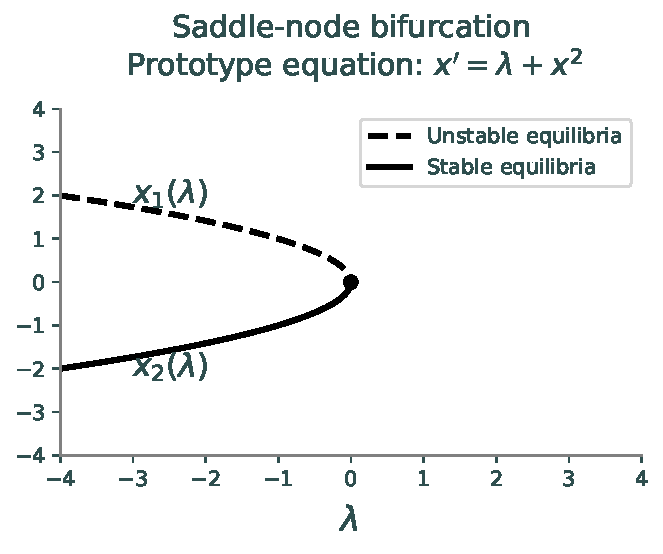
\includegraphics[width=\textwidth]{figures/SaddleNBifurcation.pdf}
\caption{Bifurcation diagram for the equation $x' = \lambda + x^2$.}
\label{bifurcation:sn}
\end{figure}

Suppose that $F(x_0,\lambda_0) = 0.$
We use a method called natural embedding to find zeros $(x,\lambda)$ of $F$ for nearby values of $\lambda$.
Specifically, we step forward in $\lambda$ by letting $\lambda_1 = \lambda_0 + \triangle \lambda$, and use Newton's method to find the value $x_1$ that satisfies $F(x_1,\lambda_1) = 0.$
This method works well except when $\lambda$ is near a bifurcation point $\lambda^*$.

The following code implements the natural embedding algorithm, and then uses that algorithm to find the curves in the bifurcation diagram for (\ref{snbifurcation}).
Notice that this algorithm needs a good initial guess for $x_0$ to get started.

\begin{figure}
\centering
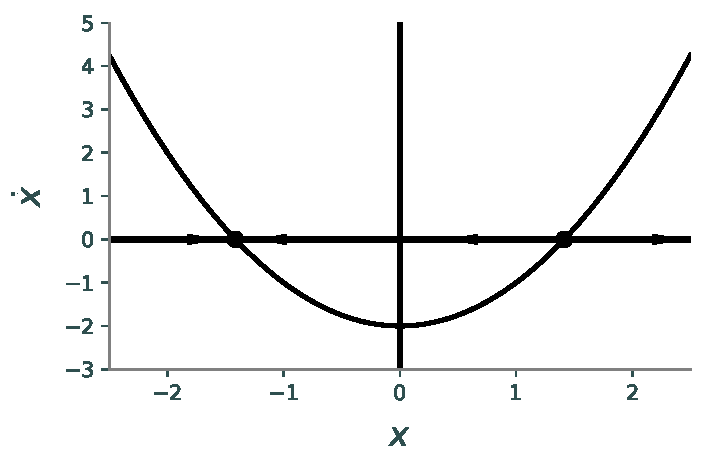
\includegraphics[width=\textwidth]{figures/SaddleNPhasePortrait.pdf}
\caption{Phase Portrait for the equation $x' = -2 + x^2$.}
\label{phaseportrait:sn}
\end{figure}

\newpage
\begin{lstlisting}
import numpy as np
import matplotlib.pyplot as plt
from scipy.optimize import newton

def embedding_alg(lams, guess, F):
    xs = list()
    for lam in lams:
        try:
            # Solve for x_value making F(x_value, param) = 0.
            x_value = newton(F, guess, args=(param,), tol=1e-7)
            # Record the solution and update guess for the next iteration.
            xs.append(x_value)
            guess = x_value
        except RuntimeError:
            # If Newton's method fails, return a truncated list of parameters
            # with the corresponding x values.
            return lams[: len(xs)], xs
    # Return the list of parameters and the corresponding x values.
    return lams, xs

def F(x, lmbda):
    return x**2 + lmbda

# Top curve shown in the bifurcation diagram
lams1, xs1 = embedding_alg(np.linspace(-5, 0, 200), np.sqrt(5), F)
# The bottom curve
lams2, xs2 = embedding_alg(np.linspace(-5, 0, 200), -np.sqrt(5), F)
\end{lstlisting}

\begin{problem}
Use the natural embedding algorithm to create a bifurcation diagram for the differential equation
\[x' = \lambda x-x^3.\]
This type of bifurcation is called a pitchfork bifurcation (you should see a pitchfork in your diagram).

Hints: Essentially this amounts to running the same code as the example, but with different parameters and function calls so that you are tracing through the right curves for this problem.
To make this first problem work, you will want to have your `linspace' run from \underline{high to low} instead of from \underline{low to high}.
There will be three different lines in this image all of which must be produced using the \li{embedding_alg} function. Any hard coding will result in an automatic 0.
See Figure \ref{prob1}.
\end{problem}

\begin{figure}[H]
\centering
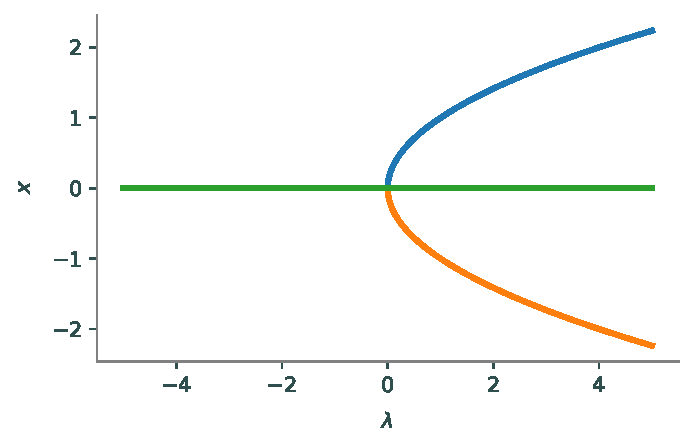
\includegraphics[width=\textwidth]{figures/prob1.pdf}
\caption{Bifurcation diagram for the equation $x' = \lambda x - x^3$.}
\label{prob1}
\end{figure}

\begin{problem}
Another useful tool for analyzing a bifurcation diagram can be to plot the trajectory of the solutions, given different parameters and initial conditions, such that the parameters chosen are from each partition of the bifurcation diagram. For example, the points
\[(\lambda, x_0)\in \left\{\left(\frac{1}{2},\frac{1}{2}\right), \left(\frac{1}{2},\frac{-1}{2}\right), \left(\frac{-1}{2},\frac{1}{2}\right), \left(\frac{-1}{2},\frac{-1}{2}\right) \right\} \]
all lie in different parts of the bifurcation diagram in Figure \ref{prob1}. We can pick a $\lambda$ and $x_0$ and find the trajectory of that points, given the ODE
\[x' = \lambda x-x^3.\]
and the initial condition $x(0)=x_0$. 
Use the four parameter value and initial condition combinations above to solve the ODE 
\[x' = \lambda x-x^3.\]
Use \li{solve_ivp} to plot on the time interval $0\leq t \leq 20$.
Be sure to include a legend.
See Figure \ref{fig:hysteresis:pitchfork_state_space}.
\end{problem}

\begin{figure}[H]
\centering
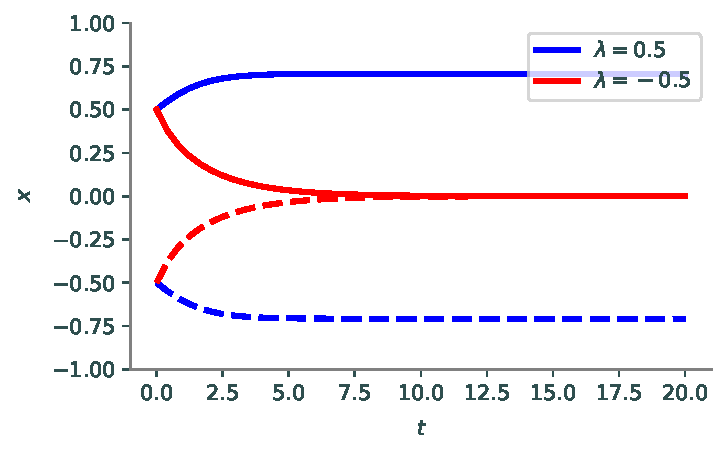
\includegraphics[width=\textwidth]{figures/pitchfork_state_space.pdf}
\caption{Possible trajectories given different $x_0$'s and $\lambda$'s for the equation $x' = \lambda x - x^3$.}
\label{fig:hysteresis:pitchfork_state_space}
\end{figure}

\section*{Hysteresis}

The following ODE exhibits an interesting bifurcation phenomenon called hysteresis:
\begin{align*}
	x' &= \lambda + x - x^3.
\end{align*}
This system has a bifurcation diagram containing what is known as a hysteresis loop, shown in Figure \ref{bifurcation:hysteresis}.
In the hysteresis loop, when the parameter $\lambda$ moves beyond the bifurcation point the equilibrium solution makes a sudden jump to the other stable branch.
When this occurs the system cannot reach its previous equilibrium by simply rewinding the parameter slightly. The next section discusses a model with a hysteresis loop.

\begin{figure}
\centering
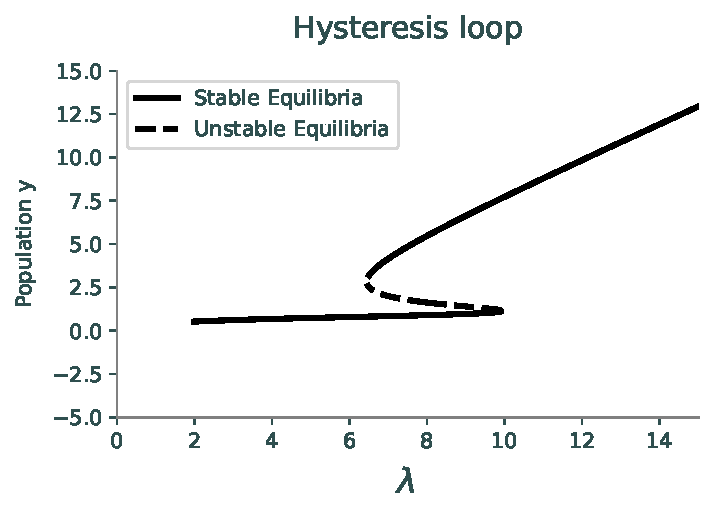
\includegraphics[width=\textwidth]{figures/HysteresisBifurcation.pdf}
\caption{Bifurcation diagram for the ODE $x' = \lambda + x - x^3$. }
\label{bifurcation:hysteresis}
\end{figure}

\begin{figure}
\centering
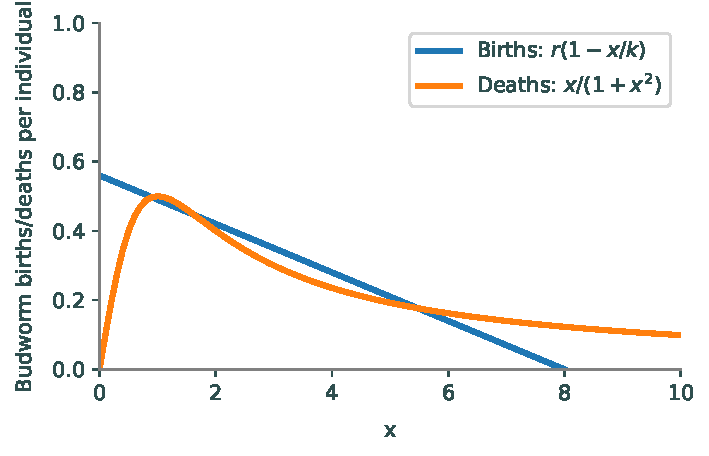
\includegraphics[width=\textwidth]{figures/BudwormEquilibria.pdf}
\caption{Graphical demonstration of nonzero equilibrium solutions for the budworm population (here $r = .56,\ k=8$); equilibrium solutions occur where the curves cross.
As $k$ increases, the line $y=r(1- x/k)$ gets more shallow and the number of solutions goes from one to three and then back to one. }
\label{equilibria:budworm}
\end{figure}

\subsection*{Budworm Population Dynamics}
Here we study a mathematical model describing the population dynamics of an insect called the spruce budworm.
In eastern Canada, an outbreak in the budworm population can destroy most of the trees in a forest of balsam fir trees in about 4 years.
The mathematical model is given by
\begin{align}
N' = RN\left(1 - \frac{N}{K}\right) - p(N). \label{budworm1}
\end{align}
This model was studied by Ludwig et al (1978), and is described well in Strogatz's text \emph{Nonlinear Dynamics and Chaos}.
Here $N(t)$ represents the budworm population at time $t$, $R$ is the growth rate of the budworm population and $K$ represents the carrying capacity of the environment.
We could interpret $K$ to represent the amount of food available to the budworms.
$p(N)$ represents the death rate of budworms due to predators (birds); we assume specifically that $p(N)$ has the form $P(N) = \frac{BN^2}{A^2 + N^2}$.

Before studying the equilibrium points of \eqref{budworm1} it is important to reduce the number of parameters in the system by nondimensionalizing.
Thus, we make the coordinate change $x = N/A$, $\tau = Bt/A$, $r = RA/B$, and $k = K/A$, obtaining finally the system
\begin{align}
	\frac{dx}{d \tau} &= rx(1-x/k) - \frac{x^2}{1+x^2}.
\end{align}

Note that $x = 0$ is always an equilibrium solution.
To find other equilibrium solutions we study the equation $r(1-x/k)-x/(1+x^2) = 0$.
Fix $r = .56$, and consider Figure \eqref{equilibria:budworm} ($k=8$ in the figure).

\newpage
\begin{figure}
\centering
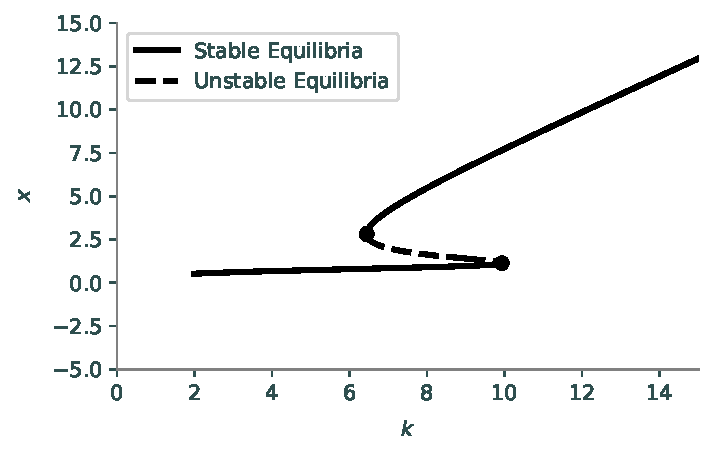
\includegraphics[width=\textwidth]{figures/BudwormPopulation.pdf}
\caption{Bifurcation diagram for the budworm population model.
The parameter $r$ is fixed at $0.56.$
The lower stable branch is known as the refuge level of the bundworm population, while the upper stable branch is known as the outbreak level.
Once the budworm population reaches an outbreak level, the available food (foliage of the balsam fir trees) in the system must be reduced drastically to jump back down to refuge level.
Thus many of the balsam fir trees die before the budworm population returns to refuge level.}
\label{bifurcation:budworm}
\end{figure}

\newpage
\begin{problem} %[Budworm Population]
Reproduce the bifurcation diagram (\ref{bifurcation:hysteresis}) for the differential equation
\begin{align*}
	\frac{dx}{d \tau} &= rx(1-x/k) - \frac{x^2}{1+x^2},
\end{align*}
where $r = 0.56$.
Be sure to include a legend.

Hint: Find a value for $k$ that you know is in the middle of the plot (i.e. where there are three possible solutions), then use the code from the previous problems to expand along each contour till you obtain the desired curve.
Now find the proper initial guesses that give you the right bifurcation curve.
The final plot will look like the one in Figure \ref{bifurcation:budworm}, but you will have to run the embedding algorithm 4-6 times to get every part of the plot. In order to make a black dashed line, add \li{'--k'} as the third argument in plt.plot() and use \li{'-k'} as the third argument in plt.plot() to get the solid black line.
\end{problem} 

\begin{problem}
Assume a time-dependent carrying capacity, defined by 
\begin{align*}	
k(t) = \begin{cases}
  8  & t \in [0,60) \\
  12  & t \in [60,150) \\
  8 & t \in [150,220) \\
  6 & t \in [220,300) \\
\end{cases}
\end{align*}
 and assume $r=0.56$ and $x(0)=x_0=0.3$. Plot the state-space diagram for the differential equation

\begin{align*}
	\frac{dx}{d \tau} &= rx(1-x/k(t)) - \frac{x^2}{1+x^2},
\end{align*}
using \li{solve_ivp} to solve the differential equation. Also plot the carrying capacity as a function of time on the same axes.
Be sure to include a legend.

Notice that returning the parameter $k$ to $8$ does not make the budworm population decrease back to the value it approached before increasing $k$ to $12$.

\end{problem} 

\section*{Two-Dimensional State Space}
The \emph{Hopf bifurcation} is one type of bifurcation that only occurs in a two- or higher-dimensional space.\footnote{\url{https://www.biodyn.ro/course/literatura/Nonlinear_Dynamics_and_Chaos_2018_Steven_H._Strogatz.pdf}}
Examples include railway vehicle stability, in which a vehicle's motion transitions from stable to unstable as speed increases.
There are two types of Hopf bifurcations: \emph{supercritical} and \emph{subcritical}.
In polar coordinates, a simple supercritical system can take the form
\begin{align}
    \begin{split}
        \label{hysteresis:eqn:2d-polar}
        r' &= \mu r - r^3 \\
        \theta' &= \omega + b r^2.
    \end{split}
\end{align}
We will be examining the effect of $\mu$ on the stability of the origin.
We restrict our analysis with the convention that $r \ge 0$.
At the origin ($r = 0$), we have $r' = 0$.
This suggests that the origin is an equilibrium, and a conversion to Cartesian coordinates confirms this (see the ``Additional Material'' section).

For $r > 0$, $\mu \le 0$ implies that $r' < 0$, so the origin is in fact \emph{asymptotically stable}.
However, something interesting happens when $\mu$ becomes positive.
In that case, we find that for $r < \sqrt \mu$ we have $r' > 0$, so the origin is unstable.
On the other hand, for $r > \sqrt \mu$ we have $r' < 0$.
This means that all trajectories not on the circle $S = \{r : r = \sqrt \mu\}$ tend toward $S$.
Moreover, on $S$ we have $r' = 0$, so trajectories on the circle will stay on it.

It turns out $S$ is a special case of a \emph{stable} limit cycle, defined by the property that nearby trajectories approach the cycle as time goes to infinity.
(The circle $S$ is special in that it attracts trajectories globally, rather than just in a neighborhood.)

\begin{problem}
    \label{hysteresis:prob:2d-state-space}
    Create an animation showing how two trajectories of the system \eqref{hysteresis:eqn:2d-polar} change as the parameter $\mu$ changes from $-0.25$ to $0.25$.
    Use 251 steps in your $\mu$-linspace.
    Use the two inital starting points $(r_0, \theta_0) = (0.1, 0)$ and $(0.6, 0)$.
    Set $\omega = b = 1$.
    Using \li{solve_ivp}, let the two trajectories evolve from $t_0 = 0$ to $t_f = 16 \pi$.
    Also plot the limit cycle (when $\mu > 0$), recalling from the above that it occurs at $r = \sqrt \mu$.
    Be sure to include a legend.
    Compare with Figure \ref{hysteresis:fig:2d-state-space}.
    Embed your animation in your notebook, and remember to push the animation as well.

    \noindent Hint: To fit the animation in the frame, it may be useful to set the plot view limits to $(-0.7, 0.7)$ (e.g., with \li{ax.set_xlim}).
\end{problem}

\begin{figure}
    \begin{subfigure}[b]{0.49\textwidth}
        \centering
        \includegraphics[width=\textwidth]{figures/hopf_mu_-025.pdf}
    \end{subfigure}
    \begin{subfigure}[b]{0.49\textwidth}
        \centering
        \includegraphics[width=\textwidth]{figures/hopf_mu_025.pdf}
    \end{subfigure}
    \caption{The solution to Problem \ref{hysteresis:prob:2d-state-space} at $\mu = -0.25$ and at $\mu = 0.25$. The points mark the initial positions of the two trajectories.}
    \label{hysteresis:fig:2d-state-space}
\end{figure}

\newpage

\section*{Additional Material}

\subsection*{Conversion of the Hopf Bifurcation System to Cartesian Coordinates}

We can convert the polar system \eqref{hysteresis:eqn:2d-polar} to Cartesian coordinates using $x = r \cos \theta$, $y = r \sin \theta$, and $x^2 + y^2 = r^2$:
\begin{align*}
    x'
    &= r' \cos \theta - r \theta' \sin \theta \\
    &= \left(\mu r - r^3\right) \cos \theta - r \left(\omega + b r^2\right) \sin \theta \\
    &= \left(\mu - r^2\right) r \cos \theta - \left(\omega + b r^2\right) r \sin \theta \\
    &= \left(\mu - \left(x^2 + y^2\right)\right) x - \left(\omega + b \left(x^2 + y^2\right)\right) y \\
    &= \mu x - x^3 - x y^2 - \omega y - b x^2 y - b y^3 \\
    y'
    &= r' \sin \theta + r \theta' \cos \theta \\
    &= \left(\mu r - r^3\right) \sin \theta + r \left(\omega + b r^2\right) \cos \theta \\
    &= \left(\mu - r^2\right) r \sin \theta + \left(\omega + b r^2\right) r \cos \theta \\
    &= \left(\mu - \left(x^2 + y^2\right)\right) y + \left(\omega + b \left(x^2 + y^2\right)\right) x \\
    &= \mu y - x^2 y - y^3 + \omega x + b x^3 + b x y^2
\end{align*}
